TRIUMF has a long history of pion branching ratio measurements \cite{Bryman3, Britton}. Each generation of experiment benefited from experience gained during the previous experiment as well as from advances in technology. The experiment that preceded PIENU was performed at TRIUMF in the 1980s and measured the branching ratio to be $(1.2265 \pm 0.0056) \times 10^{-4}$ based on $10^5$ $\pi \to e \nu$ events; the precision was dominated by systematic uncertainties.  PIENU \cite{Aguilar-Arevalo1, Aguilar-Arevalo2, Aguilar-Arevalo4, Aguilar-Arevalo5} accumulated $10^7$ $\pi \to e \nu$ events using an increased solid angle and higher resolution calorimeter, longer running time, and improvements designed to reduce systematic uncertainties. It  reported an interim result at the $0.2\%$ level given in Eq.\ref{Remu_exp} and expects to achieve $0.1\%$ precision.

The largest sources of uncertainty in these experiments have been statistics and the systematic uncertainty related to the low-energy tail correction. The statistical uncertainty for the current PIENU experiment is projected to improve by about a factor of four compared to Ref. \cite{Britton}. 
PIENU used a high-resolution ($\sigma=1\%$) crystal calorimeter consisting of a single NaI(Tl) crystal surrounded by an array of 97 pure CsI crystals. The PIENU detector is shown in Figure~\ref{fig:detector_PIENU} and described in \cite{Aguilar-Arevalo4}. The NaI crystal was 19 radiation lengths thick for on-axis decays.

\begin{figure}[h!]
\centering
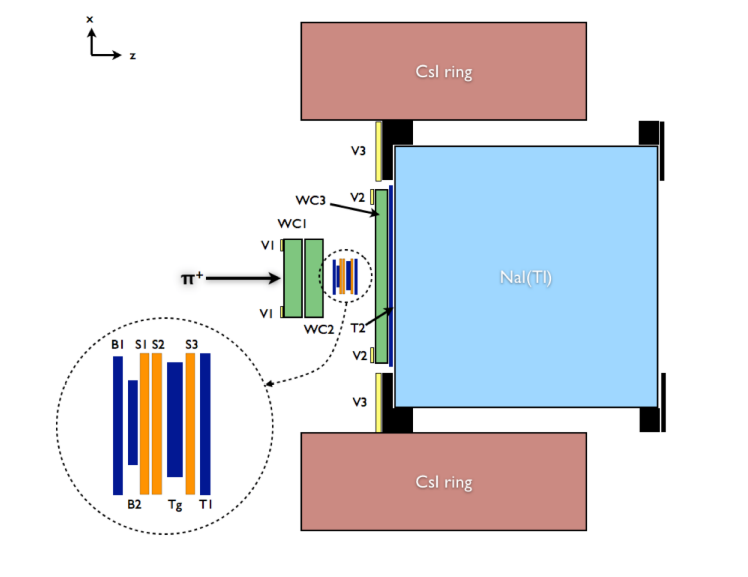
\includegraphics[scale=0.45]{sections/figures/PIENUDetector.png}
\caption{PIENU detector. Plastic scintillators are shown in dark blue, wire chambers in green, silicon strip trackers in orange, and the calorimeter in light blue and red.}
\label{fig:detector_PIENU}
\end{figure}

 PIENU obtained the branching ratio by first separating events into high- and low-energy regions at an energy cut value ($E_{cut}$) as illustrated in Fig. \ref{fig:analysis}. The time spectra were fit in each region with the $\pi^+ \rightarrow e^+ \nu$ and $\pi^+ \rightarrow \mu^+ \rightarrow e^+$ shapes, plus backgrounds originating from different sources including pion decays in flight, contamination from old muon decays etc. The raw branching ratio $R^{raw}_{e/\mu}$ was the ratio of the $\pi^+ \rightarrow e^+ \nu$ amplitude to the $\pi^+ \rightarrow \mu^+ \rightarrow e^+$ amplitude, to which corrections were subsequently applied. %By far the largest correction is the %%%%%, the most significant correction to the raw branching ratioso-called tail correction, which %%%, the most significant correction to the raw branching ratioaccounts for $\pi^+ \rightarrow e^+ %%, the most significant correction to the raw branching ratio\nu$ events with measured energy %%%, the most significant correction to the raw branching ratiobelow $E_{cut}$. 
 
\begin{figure}[h!]
\centering
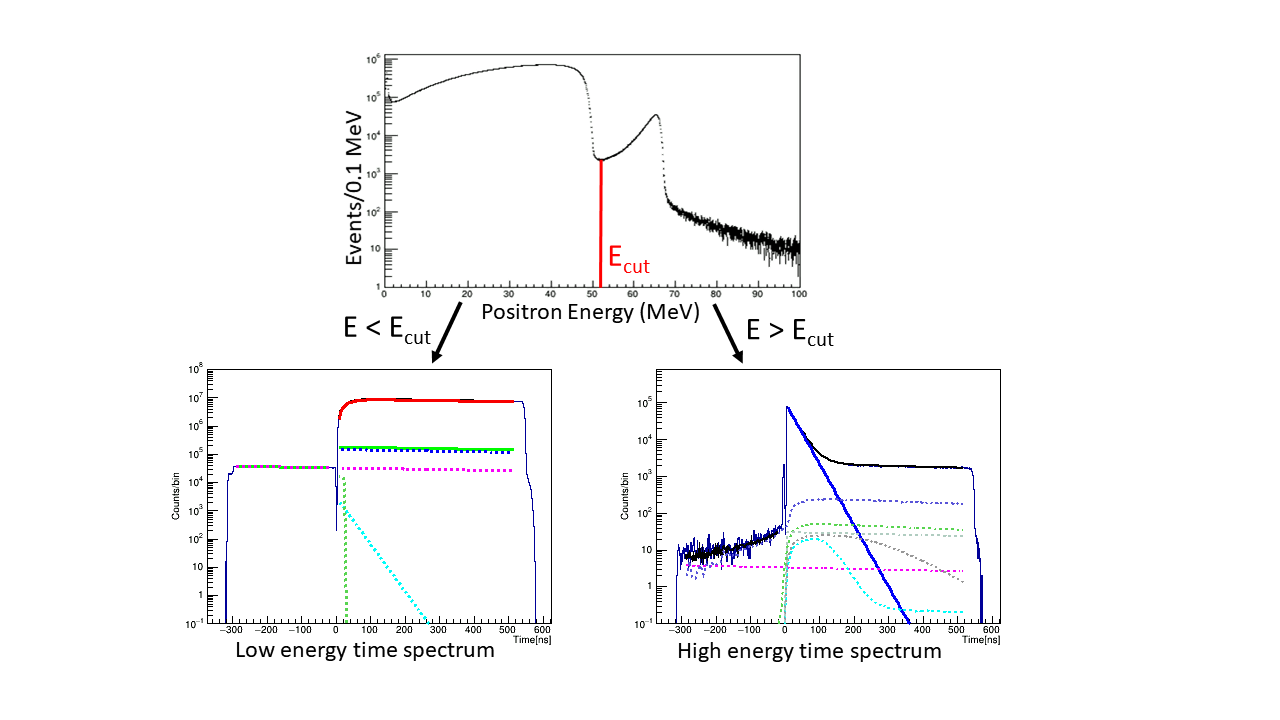
\includegraphics[scale=0.5]{sections/figures/Analysis.png}
\caption{The upper panel shows the positron energy spectrum with the red line indicating $E_{cut}$. The lower panels show the time distributions for events below and above $E_{cut}$. The black histograms are data, the red curve is the $\pi^+ \to \mu^+ \to e^+$ signal, and the blue line is the $\pi^+ \to e^+ \nu$ signal. The other histograms in various colors are the background terms.}
\label{fig:analysis}
\end{figure}

As mentioned before, several factors contributed to the size of the low energy tail, the most significant correction to the raw branching ratio. In addition to the finite energy resolution of the calorimeter and the presence of radiative decays, the positrons can lose energy on their way out of the target and before reaching the calorimeter in the non-instrumented parts of the detectors. 
%There was energy loss for positrons as they left the target and traversed material upstream of the calorimeter.  
Bhabha scattering upstream of the calorimeter can contribute to the low energy tail as well; due to the limited geometrical acceptance, secondary particles are often not absorbed by the calorimeter.  Electromagnetic showers are reasonably well contained for forward angles, but shower leakage increases at larger angles due to the reduced amount of calorimeter material.  The challenge of understanding and modeling these effects contributes to the low energy tail being the dominant source of systematic uncertainty.
%to the low energy tail in an imperfect detector means that the low-energy tail of the measured positron energy spectrum for PIENU events is the largest source of systematic uncertainty.

PIENU took special measurements to understand the response of the calorimeter, by injecting 70 MeV beam positrons into the detector at various angles. The response was highly non-uniform as a function of the angle between the positron track and the calorimeter axis; at small angles the low-energy tail was very small, but at large ($>45^\circ$) angles, it grew quickly. 
The measured energy spectrum with a beam of positrons injected along the NaI crystal axis and into the centre of the crystal, is shown in Figure~\ref{fig:0degrees_data} which displays significant bump features due to photo-nuclear effects. The details of the spectrum are discussed in \cite{Aguilar-Arevalo5}; the most important parameter is the percentage of the spectrum extending below $E_{cut}$, which in the spectrum shown is about 0.5\%. By contrast, the tail correction used in the branching ratio analysis is about 3\%, due to the effects mentioned above. A calorimeter with a similar or greater number of radiation lengths to that of the PIENU calorimeter, but covering close to the full solid angle, would not suffer from many of these effects, leading to a significant reduction in the tail correction and uncertainty.

\begin{figure}[h!]
\centering
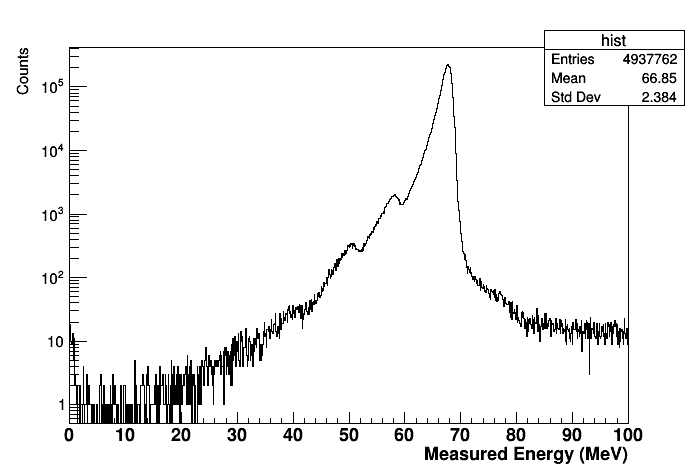
\includegraphics[scale=0.3]{sections/figures/0degrees_BINACsI.png}
%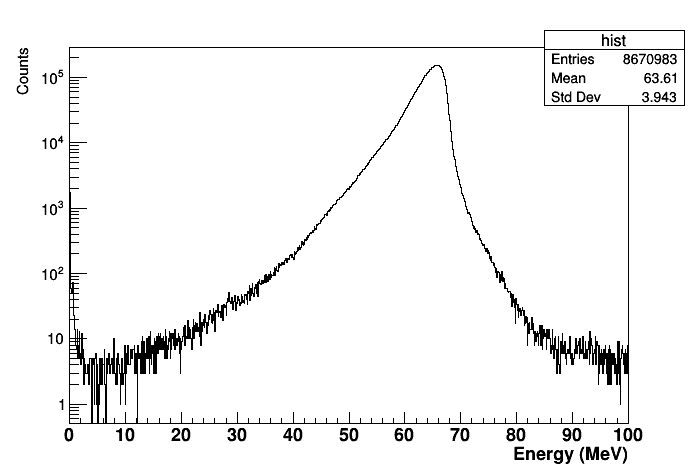
\includegraphics[scale=0.3]{sections/figures/48degrees_BINACsI.png}
\caption{Measured energy spectrum of a 70 MeV positron beam.}
\label{fig:0degrees_data}
\end{figure}

Pileup was another important source of systematic uncertainty. The usual pileup due to multiple beam particles was not severe at the relatively low beam rate of $\sim 50KHz$, and ensuring only one stopping pion at a time involved straightforward cuts in the data analysis. The much more serious pileup was a consequence of the long muon lifetime, coupled with the slow response time of the NaI(Tl) crystal. About 1\% of the muons stopped in the target lived longer than ten $\mu$s, and the long pulse width ($\sim\mu$s) of the NaI crystal raised the probability that positrons produced by such ``old muon" decays deposited energy overlapping with $\pi^+ \rightarrow \mu^+ \rightarrow e^+$ events. Such events are a background in the high-energy time spectrum, and stringent selection cuts, removing more than half the data, were employed to suppress them.  Also, ``neutral pileup" primarily from the environmental background of neutrons added energy to the calorimeter and boosted $\pi^+ \rightarrow \mu^+ \rightarrow e^+$ events into the high energy region.

The analysis of the full PIENU data set is  ongoing. A table of estimated uncertainties from  ~\cite{Aguilar-Arevalo3} is shown in Table~\ref{syst_table}.  To reach a precision of 0.01\%  all systematic effects would have to be addressed and reduced by a factor 3 to 10. The new detector concept detailed in section \ref{s:PIENUXEdet}
 addresses this challenge.  

\begin{table}[h!]
\centering
\caption{PIENU error table \cite{Aguilar-Arevalo3}.}
\label{syst_table}
\begin{tabular} {|c|c|}
\hline
Statistics & 0.19\% \\
Tail correction & 0.12\% \\
t$_0$ correction & 0.05\% \\
$\mu$ decay-in-flight correction & 0.05\% \\
Fitting parameters & 0.05\% \\
Selection cuts & 0.04\% \\
Acceptance correction & 0.03\% \\
\hline
Total & 0.25\% \\
\hline
\end{tabular}
\end{table}

 
 
